\chapter{Overkoepelende Projectstructuur}
\label{ch:overkoepelendeprojectstructuur}
In dit hoofdstuk wordt er een voorstel gedaan om de editors deel uit te laten maken van een overkoepelende projectstructuur; de editors zullen het gehele project openen in plaats van een enkel bestand. Door de editors beschikbare bestanden te laten beheren kunnen er sterkere referenties worden gemaakt tussen de game content en de editor. Een overkoepelende projectstructuur laat functionaliteiten toe die eerst niet mogelijk waren, zoals het previewen van assets in de editor en het gebruiken van gedeelde variabelen in zowel verhaal als dialoog. Om het beheren van bestanden mogelijk te maken wordt er een voorstel gedaan om de huidige folderstructuur van het NGT te veranderen. Verder worden er twee semantische lagen geïntroduceerd die de foutgevoeligheid van de nieuwe editor verminderd.

\section{Projectstructuur narrative game}
Narrative game projecten wordt ontwikkeld in het NGT. Dit template dwingt een folderstructuur af die vrijwel ieder project aanhoudt. In deze folderstructuur bevindt zich de code en content voor de game. De bestanden die samen de game content omschrijven worden ook wel ‘assets’ genoemd. Voorbeelden van assets zijn: afbeeldingen, video’s, geluidsbestanden en configuratie bestanden. Kortom, alle media en data die het spel (in)direct aan de speler toont. Vaak worden deze assets al geordend in mapjes wat al wijst op een behoefte aan een projectstructuur.

\section{Koppeling tussen assets en de editors}
De huidige editors openen een save-bestand. Voor de story editor is dit een ‘.sty’ bestand, de dialog editor opent een ‘.dlg’ bestand. Beide schrijven het export-bestand weg naar een los JSON-bestand. Assets worden handmatig gespecificeerd in een aparte JSON, ook wel assets.json genoemd (zie bijlage \autoref{app:assetsjson}). Beide editor refereren naar assets door middel van een sleutel die correspondeert met een sleutel in de assets.json. 

Dit betekent dat de editors niks af weten van de assets in het project. Er is een folder vol assets die allemaal worden ingeladen. Deze selectie ingeladen assets kunnen worden verwerkt in verhaal of dialoog. Er zijn use cases voor een overkoepelende projectstructuur opgesteld en gevalideerd in de wekelijkse meetings met de bedrijfsbegeleider en opdrachtgever (bijlage \autoref{app:usecasesprojectstructuur}). Hieruit blijkt dat het gebruikt van onbeheerde assets invloed heeft op de foutgevoeligheid, efficiëntie en functionaliteit van de editors. 

\subsection{Foutgevoeligheid}
Content typen met referenties naar assets, zoals ‘image content’ welke refereert naar een image asset, zijn erg gevoelig voor menselijke fouten. Deze content typen tonen voor iedere referentie een invoerveld die één lijn aan tekst bevat. Hierin kunnen gebruikers de sleutel invoeren die bij de juiste asset hoort. De invoer kan niet worden gecontroleerd door de editor wat twee problemen introduceert. Typefouten of referenties naar niet bestaande assets worden toegelaten. Hiernaast wordt het invoeren van verkeerde typen assets toegestaan. Zo zou ‘image content’ een referentie kunnen bevatten naar een mp3-bestand. De editor kunnen geen semantiek toewijzen aan assets.

Beide scenario’s worden niet afgevangen in de editors en kunnen resulteren in ongewenst gedrag en mogelijke crashen in de game. Dit hakt in op de efficiëntie van de editors.

\subsection{Inefficiëntie}
De foutgevoeligheid haakt in op de efficiëntie van de editors. Door een foutgevoelige editor moeten er meer testen en eventuele correcties uitgevoerd worden om een stabiele game aan te kunnen leveren.
Hiernaast is er geen mogelijkheid om ongebruikte assets te filteren, ongebruikte assets blijven altijd in de game zitten. Sommige hiervan zullen zelfs worden ingeladen als ze in het JSON-bestand staan. Dit zorgt voor een langere en onnodige laadtijd van de game.

\subsection{Disfunctionaliteit}
Zoals beschreven in \autoref{ch:technologystack}, speelt klant co-creatie een rol in de toekomst van de editor. Hiervoor is het belangrijk dat de editors beschikken over een sterke visualisatie van het verhaal\cite{Schipper2015}. Dit is lonend voor zowel klant als game design. Deze visualisatie moet naast overzicht ook inzicht bieden in de game content, zo zal ‘image content’ een preview moeten laten zien van de gerefereerde afbeelding. Om dit mogelijk te maken moet er enigszins sprake zijn van een overkoepelende projectstructuur waarbij assets beheerd worden door de editor. 


\section{Behoefte aan een overkoepelende projectstructuur}
Door mee te werken aan een narrative game project kwamen er enkele behoeftes naar boven. In de wekelijkse meetings zijn deze gevalideerd en aangevuld. Hieruit zijn use cases opgesteld (zie bijlage \autoref{app:usecasesprojectstructuur}) die gebruikt worden om de behoefte aan een overkoepelende projectstructuur naar voren te brengen. 

\begin{wrapfigure}{r}{0.35\textwidth}
    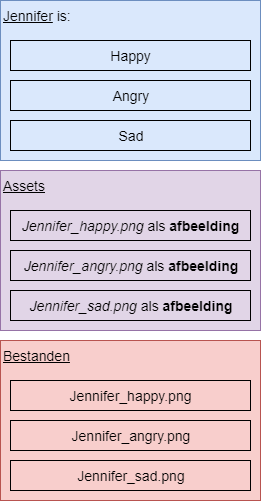
\includegraphics[width=0.33\textwidth]{SemanticLayersWithoutArrows}
    \caption{De verschillende asset betekenis lagen.}
    \label{fig:semanticgamecontentlayersdetailed}
    \centering
\end{wrapfigure}

In een digitale interactive narratief wordt er gebruik gemaakt van variabelen om conditionaliteit mogelijk te maken. Het beschikken over gedeelde variabelen tussen verhaal en dialoog is nodig om het verhaal te kunnen sturen volgens gemaakte keuzes in de dialoog en wederzijds. Deze gedeelde variabelen worden gezien als een overkoepelend construct en wekt de vraag naar een overkoepelende projectstructuur op waarbij variabelen, verhalen en dialogen samen komen en met elkaar verbonden worden.

Het kan vervelend worden ondervonden om gebruik te moeten maken van twee verschillende applicaties die op veel fronten overlappen. Voor het verhaal maakt men gebruik van de story editor, voor dialogen de dialog editor. Een overkoepelende projectstructuur maakt het mogelijk om verhaal en dialoog bestanden met elkaar te verbinden. Naast story telling tools kunnen ook integrated development environments (IDE's) gebruik maken van een overkoepelende projectstructuur. In veel IDE's is dit terug te zien aan de ingebouwde verkenner, waarin de gebruiker bestanden kan selecteren en openen.

Referenties naar assets worden gemaakt door het invoeren van een tekstuele sleutel. Daarbij moet de asset worden gespecificeerd in het assets JSON-bestand. Dit is relatief makkelijk te vergeten en daarnaast worden er veel typfouten gemaakt. Daarnaast kan de gebruiker zonder waarschuwing een verkeerd type asset invoeren, zoals een afbeelding in een geluid veld. De editor moet een lijst aanreiken met beschikbare assets van het juiste type, om zo de foutgevoeligheid te verminderen.

Naast het onderscheid maken tussen typen assets is het wenselijk om entiteiten te kunnen koppelen aan assets. Hierbij bestaat bijvoorbeeld een karakter uit meerdere emoties die uitgedrukt worden in afbeeldingen (\autoref{fig:semanticgamecontentlayersdetailed}).

\section{Stappen richting een overkoepelende projectstructuur}
Om aan deze behoeftes te voldoen moeten er stappen worden gezet richting een overkoepelende projectstructuur. De editor moet hiervoor bij bestanden kunnen die zich bevinden in de projectfolder. Wat betekend dat de editor de gehele projectfolder zal moeten openen in plaats van alleen het save-bestand. De folderstructuur van het project moet dit wel ondersteunen; bruikbare assets moet gescheiden worden van niet bruikbare bestanden zoals code. Daarnaast moet er een folder komen waarin alle overkoepelende constructen, zoals variabelen en content typen schema's, worden opgeslagen.

De editor moet bestanden in de projectfolder inventariseren en onderscheid maken tussen zowel bruikbare bestanden als typen bestanden. Daarnaast moet er een manier komen om assets te koppelen aan entiteiten. Wanneer bestanden worden verplaatst, aangepast of verwijderd worden moet de inventarisatie en referenties naar deze assets worden geüpdatet als nodig.

Het afdwingen van typen assets in de inspector vereist een uitbreiding van JSON-schema. In het schema moet het type asset kunnen worden gedefinieerd.

Tenslotte zal moeten worden gekeken naar het exporteer proces van game content. Hierin zal er een pakketje moeten worden gemaakt waarin zich alle game content bevindt.

\section{Een ondersteunende folderstructuur}
In een overkoepelende projectstructuur wordt de gehele project folder geopend in plaats van een specifiek bestand. Door de project folder te openen kunnen assets binnen het project geïnventariseerd en beheerd worden. Hiernaast kan de inventarisatie aangepast worden als er assets verwijderd of toegevoegd worden. In \autoref{sec:assetmanagement} wordt er dieper in gegaan op het beheren van assets.

Bij het openen van de gehele project folder is het alleen wenselijk om assets te beheren die verwerkt kunnen worden in het verhaal. Bestanden die broncode of configuraties voor command line tools representeren kunnen niet worden verwerkt in het verhaal. De editor hoeft niks van deze bestanden af te weten. In de huidige folderstructuur van het ‘narrative game template’ (NGT), het raamwerk waarin narrative games gerealiseerd worden, bevinden zich bruikbare en niet bruikbare bestanden in deze zelfde folder. Om een gestructureerde overkoepelende projectstructuur toe te laten zullen er aanpassingen moeten worden gedaan op de folderstructuur. Deze aanpassing zijn alleen bedoelt om een overkoepelende projectstructuur te ondersteunen.

\section{Folderstructuur van het narrative game template}
In \autoref{fig:ngtfolderstructure} wordt de folderstructuur van het NGT weergeven. De ‘src’ (source) directory bevat de broncode en game content van de game. Hierin bevinden zich een ‘assets’ en een ‘ranj’ directory. De ‘ranj’ directory bevat de broncode van het spel en zal dus geen deel uit moeten maken van de overkoepelende projectstructuur. In de ‘assets’ directory zitten, zoals de naam luidt, alle asset die worden verwerkt in de game. Hiernaast bevinden zich project specifieke configuraties en flash files\footnote{Visual designers gebruikt Adobe Animate CC om schermen te ontwikkelen voor narrative games.} ook in deze directory. Deze project specifieke configuraties en flash files zijn niet verwerkbaar in het verhaal en moeten dus uit de assets directory. Project specifieke configuraties zouden eventueel wel gebruikt kunnen worden door de editors. Een voorbeeld hiervan is het content typen dataschema beschreven in \autoref{ch:diversiteitingamecontent}. 

Dit creëert de behoefte voor een nieuwe directory genaamd ‘ProjectSettings’. Hierin zullen zich project specifieke configuratie bestanden bevinden. Waarbij sommige bestanden, zoals het content typen dataschema, uitgelezen zal worden door de editors. Dit maakt het definiëren van een selectie aan project specifieke content typen op projectniveau mogelijk.

\begin{figure}[htb]
    \dirtree{%
    .1 /.
    .2 autoplay.
    .2 build-tools.
    .2 dev-tools.
    .2 src.
    .3 assets.
    .3 css.
    .3 lib.
    .3 ranj.
    .3 swf.
    .3 test.
    .2 translations.
    }
    \caption{Folderstructuur van het NGT.}
    \label{fig:ngtfolderstructure}
\end{figure}

\section{Het beheren van assets}
\label{sec:assetmanagement}
Om de assets te beheren zal de editor een lijst moeten bijhouden met daarin informatie over beschikbare assets in de ‘assets’ directory. Elementen in deze lijst worden gerepresenteerd als:
\begin{quote} 
    \centering    
    \textit{
        \{ id : string, path : string, type : string \} 
    }
\end{quote}
\noindent Waar;
\begin{description}
    \item[id] bestaat uit een unieke string die eenmaal gegeneerd zal worden wanneer de asset geïnventariseerd wordt. Deze wordt gebruikt om naar assets te refereren. Dit speelt een rol in het exporteer proces beschreven in \autoref{sec:exportproces}.
    \item[path] een relatief pad naar de asset vanaf de root van het project is. Zo kan zowel de editor als het NGT de locatie van de asset achterhalen. Wanneer er naar deze asset gerefereerd wordt kan de bestandsnaam uit dit pad getoond worden om inzicht te geven in de gerefereerde asset.
    \item[type] semantiek toekent aan de asset (e.g. ‘image’, ‘sound’).
\end{description}

Door gebruik te maken van een ‘id’ blijven referenties intact wanneer het pad naar het bestand veranderd. Als de asset verwijderd wordt zullen referenties naar deze asset breken. De editor kan vervolgens aangeven welke referenties gebroken zijn en eventueel vragen met welke asset deze vervangen moeten worden. Een nadeel aan het gebruik van een onleesbare sleutel is dat de assets niet statisch opgehaald kunnen worden in het NGT. Het NGT kan sleutel uitlezen uit het exporteer bestand en deze omzetten naar de afbeelding (zie \autoref{sec:exportproces}), maar een programmeur kan geen afbeelding inladen door een statische sleutel mee te geven. Als dit wel wenselijk is zou er eventueel een ‘tag’ property kunnen worden toevoegt aan de elementen in de lijst. Deze zou dan wel handmatig moet worden ingesteld in de editor, wat een user interface zal vereisen.

Deze lijst zal tijdens de eerste keer opstarten van de editor opgebouwd en weggeschreven worden naar een JSON-bestand in de ‘ProjectSettings’ folder. Wanneer de lijst aanwezig is in de ‘ProjectSetting’ zal deze worden ingeladen tijdens het opstarten van de editor.

Om de lijst bij te houden terwijl de editor open is zal de ‘assets’ folder worden ‘gewatched’. Dit houdt in dat de editor een event afvuurt wanneer er een bestand aangemaakt, bewerkt, verplaatst of verwijderd wordt. NodeJS beschikt over een module genaamd ‘filesystem’ die deze functionaliteit aanbied. Daarentegen blijkt deze functionaliteit van NodeJS vrij inconsistent is, dit meldt NodeJS ook in de documentatie\cite{NodeDocFS}. Met twee events, zijnde ‘change’ en ‘rename’, is het lastig om te achterhalen wat precies het event afvuurde. 

Er kan gebruik gemaakt worden van een library, zoals Chokidar\footnote{https://github.com/paulmillr/chokidar}, die meer consistentie biedt. Deze library biedt een interface met expliciete events zoals ‘add, ‘change’ en ‘unlink’. Hiernaast zijn er ook events voor directory beschikbaar zoals ‘addDir’ en ‘unlickDir’. Chokidar wordt gebruikt in veel projecten\footnote{https://www.npmjs.com/browse/depended/chokidar}, waaronder Microsoft’s visual studio code\footnote{https://github.com/microsoft/vscode}. 

\subsection{Optimalisatie}
\label{subsec:optimalisationformat}
Het refereren naar assets is een veel voorkomende actie in de editors. Wanneer de gebruiker in ‘image content’ naar een afbeelding wilt refereren zal de lijst gefilterd moeten worden op assets met het type ‘image’ (\autoref{lst:filterassetimage}). Het iedere keer moeten filteren van een potentiele grote lijst aan assets kan mogelijk, afhankelijk van de grootte van de lijst, zorgen voor een slechte gebruikerservaring. De tijdcomplexiteit van het algoritme in \autoref{lst:filterassetimage} kan worden uitgedrukt als \textit{O(n)}, waarin ‘n’ het aantal elementen in de array zijn. 

\begin{figure}[htb]
    \centering
    \lstset{language=JavaScript}
    \begin{lstlisting}
    availableAssets.filter(asset => asset.type === 'image');
    \end{lstlisting}
    \caption{Het filteren van assets met het type 'image'.}
    \label{lst:filterassetimage}
\end{figure}

Om het vinden van assets met een bepaald type efficiënter te maken kan de editor een JavaScript object bijhouden die dient als een ‘lookup table’. In dit object dienen de properties als keys die ieder een array van assets bevatten met dat type (zie \autoref{lst:optimizedmanageformat}). De tijdcomplexiteit van een property lookup zoals in \autoref{lst:propertylookup} kan worden uitgedrukt als \textit{O(1)}.

\begin{figure}[htb]
    \centering
    \lstset{language=JavaScript}
    \begin{lstlisting}
    {
        images: [
            ..
        ],
        videos: [
            ..
        ]
    }
    \end{lstlisting}
    \caption{Geoptimaliseerd formaat voor het beheren van assets.}
    \label{lst:optimizedmanageformat}
\end{figure}

\begin{figure}[htb]
    \centering
    \lstset{language=JavaScript}
    \begin{lstlisting}
    const availableImages = availableAssets.images;
    \end{lstlisting}
    \caption{Het verkrijgen van alle beschikbare images door middel van een property lookup}
    \label{lst:propertylookup}
\end{figure}

\section{Semantiek binden aan assets}

\begin{wrapfigure}{r}{0.35\textwidth}
    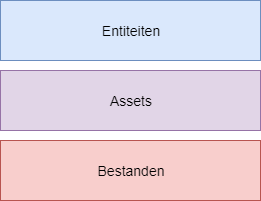
\includegraphics[width=0.33\textwidth]{SemanticLayersInGameContent}
    \caption{Semantische lagen in game content.}
    \label{fig:semanticgamecontentlayers}
    \centering
\end{wrapfigure}

Om de editors minder foutgevoelig te maken wordt er semantiek in de vorm van een type toegewezen aan de assets. Zo moeten de nieuwe editors alleen het gebruikt van afbeeldingen in ‘image content’ toelaten. Door een type toe te wijzen aan assets kunnen types worden afgedwongen in de editor. 

In deze paragraaf is er sprake van twee semantische lagen boven die gebonden worden aan bestanden die beschikbaar zijn voor de editor: de asset- en entiteiten laag. De asset laag classificeert bestanden op bestandstypen zoals afbeelding of video. De entiteiten laag categoriseert en koppelt deze assets aan hogere constructen zoals karakters en locaties. 

Voor de eerste semantische laag, het hangen van types aan bestanden, moeten de volgende stappen worden ondernomen:

\begin{enumerate}
    \item De nieuwe editor moet een type kunnen hangen aan bestanden wanneer deze ingeladen worden.
    \item Het content typen dataschema moet typen kunnen \item De inspector moet het afgedwongen typen in het dataschema respecteren en eventuele andere typen weigeren.
\end{enumerate}

Boven op de assets laag wordt de entiteiten laag gebouwd.

\begin{enumerate}[resume]
    \item Assets moeten gecategoriseerd en gekoppeld kunnen worden aan hogere constructen.
\end{enumerate}

\subsection{Bestanden koppelen aan een type}
Er kan een type aan een assets gekoppeld worden door de extensie van het bestand te respecteren. Zo is een ‘.png’ of ‘.jpeg’ een afbeeldingen en een ‘mp4’ een video. Deze semantische laag wordt vanaf nu de ‘asset laag’ genoemd. De nieuwe editor zal in code over een map moeten beschikken waarin een bestand extensie gekoppeld staat aan een type. Alleen extensies die ondersteund worden door het NGT zullen moeten worden opgenomen in deze map. Deze map wordt gedefinieerd in broncode, omdat deze wordt geacht om statisch te zijn. Als de map aangepast moet worden zal de programmeur dit moeten doen, omdat hier verdere consequenties aanhangen. Het toevoegen van een nieuwe mapping zal invloed hebben op het NGT, deze moet de nieuwe extensie ondersteunen. Hiernaast zal het omzetten van een mapping moeten resulteren in een migratie van de interne lijst aan beheerde assets.

\subsection{Het uitbreiden van JSON-schema functionaliteit}
Het content typen dataschema moet uitgebreid worden om informatie over het type asset te verstrekken. Refereren naar assets gebeurd door middel van een sleutel; de ‘id’ waarde van de elementen in de lijst. Een sleutel is een string wat betekend dat het JSON-schema voor een referentie property nog steeds ‘string’ waarde voor het ‘type’ keyword bevat. Er moet een keyword toegevoegd worden om metadata te verstrekken over het type asset.

JSON-schema verstrekt zelf al een ‘format’ keyword die semantische validatie toelaat. Een voorbeeld van een formaat is: ‘email’\cite{Droettboom2016}. De waardes van format mogen uitgebreid worden naar benodigde formaten. Maar omdat een ‘id’ niet in een onderscheidbaar formaat staat is het beter om een nieuw keyword toe te voegen waarin het type asset omschreven kan worden. Hiervoor wordt er een nieuw keyword geïntroduceerd: ‘assetType’. Voorbeelden van waardes van dit keyword zijn: ‘image’, ‘video’, ‘sound’, ect ...

\subsection{Het afdwingen van typen in de inspector}
Om JSON-schema’s te reflecteren in de inspector wordt gebruik gemaakt van de ‘react-jsonschema-form’ library, zoals vermeld in \autoref{ch:diversiteitingamecontent}. Het toevoegen van een nieuw keyword in het JSON-schema woordenboek betekend dat er nieuwe componenten gemaakt moeten worden die dit keyword ondersteunen. Deze component moet getoond worden wanneer het ‘assetType’ keyword aanwezig is in het schema.

Het ondersteunen van dit nieuwe keyword heeft een grote impact op de library. Om het ‘assetType’ keyword te ondersteunen moet het standaard gedrag van de library worden aangepast; het standaard veld voor een string type moet worden overschreven. De component die het string veld overschrijft zal de juist component teruggeven voor het schema.

\pagebreak

\subsection{Het koppeling van assets aan entiteiten}
Vaak worden afbeeldingen van karakters en locaties geordend in een folderstructuur. Dit duidt op een behoefte aan het categoriseren van assets. Met een tweede semantische laag worden asset van hetzelfde typen handmatig gebonden aan hogere entiteiten zoals karakters en locaties. Hiermee kan worden voorkomen dat er per ongeluk een verkeerde afbeelding bij een bepaald karater wordt gebruikt.

Omdat het refereren naar assets gaat via een menselijk onleesbare sleutel zal het handmatig binden van assets aan entiteiten moeten gebeuren door middel van een user interface in de editors. Deze user interface zal de gebruiker meer informatie geeft over de asset waarmee de gebruiker deze asset kan identificeren. Wanneer deze gekoppeld wordt aan een entiteit zal de editor de bijbehorende sleutel zoeken.

Deze semantische laag leeft niet in het content typen schema zoals de eerste semantische laag, maar op project niveau. Een geserialiseerd (zoals te zien in \autoref{lst:serializedentitylayer}) formaat zal dan ook worden opgeslagen in de ‘ProjectSettings’ folder. Het geserialiseerde formaat in \autoref{lst:serializedentitylayer} is geoptimaliseerd zoals beschreven in \autoref{subsec:optimalisationformat}.

\begin{figure}[htb]
    \centering
    \lstset{language=JavaScript}
    \begin{lstlisting}
    {
        "images": [
            {
                "jennifer": [
                    "idAsset1",
                    "idAsset2"
                ]
            }
        ],
        "videos": [
            ..
        ]
    }          
    \end{lstlisting}
    \caption{Geserialiseerde representatie van de entiteiten laag.}
    \label{lst:serializedentitylayer}
\end{figure}

\begin{wrapfigure}{r}{0.42\textwidth}
    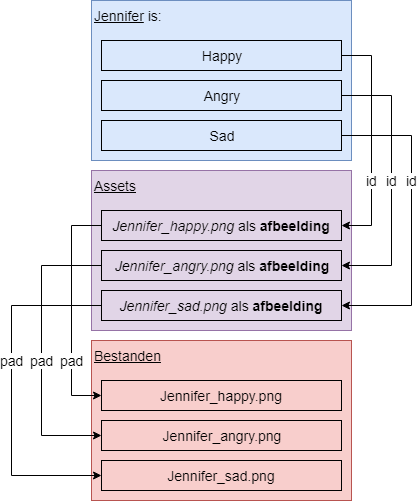
\includegraphics[width=0.4\textwidth]{EntityLayerExample}
    \caption{Relaties tussen de verschillende semantische lagen.}
    \label{fig:semanticlayerrelationships}
    \centering
\end{wrapfigure}

Vervolgens zullen content typen met een referentie naar een asset een extra veld moeten tonen in de inspector. Dit extra veld is een drop down menu waarin een keuze gemaakt kan worden uit de eerder gecreëerde entiteiten. Vervolgens kunnen de assets gefilterd worden op de geselecteerde entiteit. Dit extra veld wordt niet gedefinieerd in het content typen schema en niet geëxporteerd. Het wordt wel opgeslagen in de save file die de editor produceert.

De relaties tussen de semantische lagen zijn terug te zien in \autoref{fig:semanticlayerrelationships}.

\clearpage
\section{Het exporteren van game content}
\label{sec:exportproces}
Voorheen exporteerde de huidige editors slechts twee bestanden die het verhaal en gelokaliseerde inhoud omschreven. Een overkoepelende projectstructuur maakt het mogelijk om gebruikte assets, het verhaal en configuratie bestanden samen te bundelen in een archief format zoals tar\footnote{https://www.freebsd.org/cgi/man.cgi?query=tar\&apropos=0\&sektion=5\&manpath=FreeBSD+7.0-RELEASE\&arch=default\&format=html} of asar\footnote{https://github.com/electron/asar}. Er is niet gekeken naar een “best passende formaat” in deze context. Naast dat dit het laden van ongebruikte assets voorkomt verkleint dit het aantal HTTP requests, die gemaakt moeten worden om alle files binnen te halen. Een HTTP request bevat extra informatie welke iedere keer mee gestuurd zal worden\cite{Fielding1999}. Dit maakt het ophalen van één groter bestand sneller dan vele kleinere bestanden wat zorgt voor een snellere laadtijd van het spel.

Het NGT maakt gebruik van een library genaamd: ‘preloadJS’\footnote{https://www.createjs.com/preloadjs}. Met deze library worden bestanden ingeladen. De library biedt de mogelijkheid om een zogenaamde ‘manifest’ op te stellen. Dit is een JSON-bestand waarin paden naar bestanden worden gekoppeld aan een sleutel. De nieuwe editor kan een manifest specificeren, omdat deze beschikt over de sleutels en paden van gebruikte assets. Paden naar assets worden gestript van (sub)directories die zich bevinden in het pad, zodat alleen de bestandsnaam met extensie overblijft. Vervolgens wordt het basis pad gespecificeerd door de export locatie te pakken en de locatie van het NGT project hiervan af te trekken. Dit resulteert in een relatief pad dat het NGT leidt naar de locatie van de assets. Een voorbeeld van een manifest is terug te zien in \autoref{lst:manifestexamplepreloadjs}. Omdat dit proces zo alleen zou werken voor de ‘preloadJS’ library is het aan te raden om voor het genereren van een manifest gebruik te maken van het ‘strategy design pattern’, om zo ondersteuning voor eventuele andere libraries te bieden.

\begin{figure}[htb]
    \centering
    \lstset{language=JavaScript}
    \begin{lstlisting}
    {
        "path": "assets/",
        "manifest": [{
                "id": "8e3c642d-ab1e-4c81-a379-0b236bf692f8",
                "src": "jennifer_happy.png"
            },
            {
                "id": "23951903-0f4e-43d2-9602-5fd6e70b0d32",
                "src": "jennifer_angry.png"
            }
        ]
    }               
    \end{lstlisting}
    \caption{Voorbeeld van een manifest in preloadJS.}
    \label{lst:manifestexamplepreloadjs}
\end{figure}

\pagebreak
\section{Conclusie}
Met deze conclusie wordt deelvraag “Hoe kan game content in een overkoepelende projectstructuur verbonden en geordend worden?“ beantwoord.

Het gebruiken van een overkoepelende projectstructuur in de nieuwe editors bevorderd efficiëntie, functionaliteit en verminderd foutgevoeligheid. De folderstructuur van het NGT zal aangepast moeten worden om deze overkoepelende projectstructuur te ondersteunen.

Om game content te ordenen en met elkaar te verbinden in een overkoepelende projectstructuur zal de editor assets, bestanden die samen de game content opbouwen, moeten beheren. Dit wil zeggen dat de nieuwe editor een lijst met beschikbare assets zal bijhouden. Elementen in deze lijst bestaan uit een gegenereerde “menselijk onleesbare” unieke sleutel, een pad naar het bestand en het type bestand (e.g. afbeelding) die semantiek toe kent aan de asset. De sleutel maakt het verbinden van assets mogelijk. Deze sleutel wordt gebruikt om te refereren naar de bijbehorende asset en zorgt dat referenties niet breken wanneer de asset verplaatst wordt. Een nadeel aan een menselijk onleesbare sleutel is dat alleen de editor kan refereren naar deze assets. De programmeur kan moeilijk refereren naar deze assets vanuit statische context. Bij iedere verandering in de lijst zal deze worden geserialiseerd en weggeschreven naar een bestand in de overkoepelde project folder, zodat deze uitgelezen kan worden wanneer de editor het project opent. Als dit bestand wordt verwijderd zullen alle referenties binnen de editors breken.

Semantiek wordt toegekend aan de assets door (1) automatisch een type te binden aan assets door middel van de bestandsextensie en (2) een handmatige stap waarbij assets aan entiteiten gebonden worden. Een voorbeeld van een entiteit is een karakter welke bestaat uit verschillende afbeeldingen die emoties representeren.

Wanneer de nieuwe editor het verhaal exporteert zullen alle gebruikte assets, configuratie bestanden en het verhaal samen gebundeld worden in een archief format zoals tar. Dit verminderd het aantal HTTP requests dat het NGT hoeft te maken om assets in te laden. Het NGT gebruikt de library ‘preloadJS’ om bestanden in te laden. Deze heeft een manifest nodig die opgesteld moet worden tijdens de exporteer stap.

\section{Vervolgonderzoek}
\subsection{User interfaces voor beheren van de entiteiten laag}
Het binden van assets aan entiteiten is een handmatig proces waarbij de gebruiker via een user interface assets moet kunnen koppelen aan (zelf aangemaakte) entiteiten. Hiervoor dient de gebruiker over een user interface te beschikken waarbij de gebruiker assets kan koppelen aan entiteiten, omdat het lastig is om te werken met menselijk onleesbare asset sleutels. Er is geen onderzoek gedaan naar hoe deze user interface met werken en eruit moet zien. Dit lijkt een behoefte voor een verkenner in de editors op te roepen die gebruikt kan worden om bestand te inspecteren. De user interface voor de koppeling tussen assets en entiteiten zou eventueel op dezelfde plek kunnen komen als de inspector, wanneer er een bestand geïnspecteerd wordt.

\subsection{Exporteer formaat}
De overkoepelende projectstructuur maakt het mogelijk om gebruikte assets, configuraties en het verhaal te archiveren in een formaat zoals tar. Er zou nog onderzoek gedaan moeten worden naar verschillende archief formaten en hun voor- en nadelen. Vervolgens moet er gekeken worden naar hoe het NGT deze kan uitpakken/ uitlezen.